\section{Overview of the Solution}

\subsection{States}

\subsubsection{Modes}

The program has two main modes. These are Piano and Playback.
\textbf{SW0} is pressed to switch between the different states.
%To switch between state the \textbf{SW0} is pressed.

\begin{figure}[h]
  \centerline{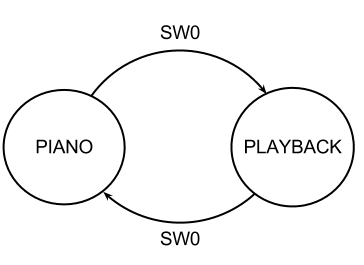
\includegraphics[width=150px]{mode.png}}
  \caption{State diagram for modes}
  \label{modestates}
\end{figure}

\subsection{Interrupt Routines}
The program is heavily centered around the two interrupt routines, button\_isr and abdac\_isr, found in
\textbf{interrupt.c}.

\subsubsection{Button Interrupt Routine}
The button routine is responsible for switching betweens the modes shown in Figure[\ref{modestates}].
If the mode is Piano it saves the button state for the abdac routine. If the mode is Playback it initializes
the next sample to be played.
\begin{figure}[h]
  \centerline{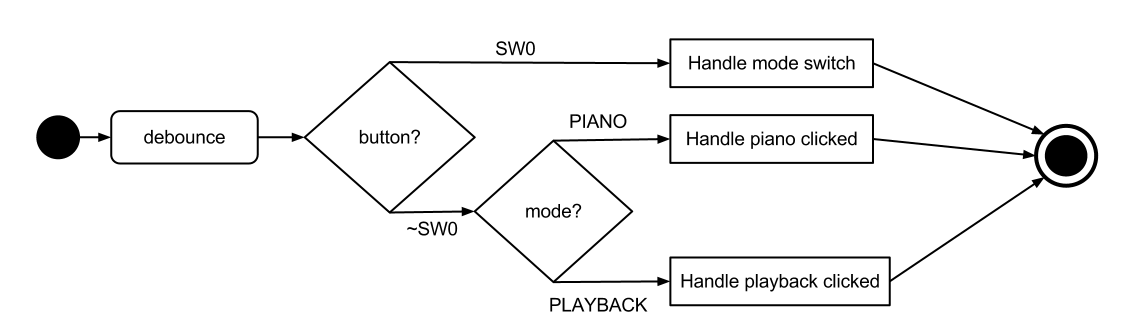
\includegraphics[width=400px]{button_isr.png}}
  \caption{State diagram for buttons}
\end{figure}
\newpage
\subsubsection{ABDAC Interrupt Routine}
The ABDAC routine behavior depends on the the mode. It delegates the work of setting up the next sample
to either the Piano or Playback module and ask the gpio to write to the abdac.

\begin{figure}[h]
  \centerline{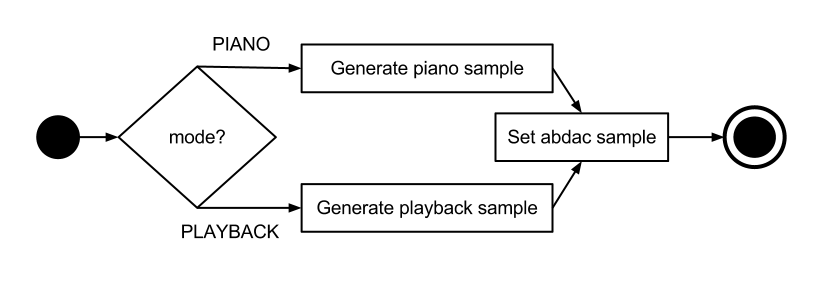
\includegraphics[width=400px]{abdac_isr.png}}
  \caption{State diagram for abdac}
\end{figure}


\subsection{Datastructures}

In order to play sounds the sound samples has to be saved. A sample contains four tracks where each track
is a series of notes in a linked list.

\subsubsection{Note structure}
A musical note is represented in the program by the datatype note\_t defined in \textbf{note.h}.
\begin{figure}[h]
  \centerline{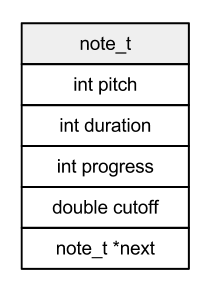
\includegraphics[width=80px]{note_t.png}}
  \caption{Datatype for notes}
\end{figure}

This type is used as a linked list to produce a track. The pitch is a number which relates to the frequency
of the note. Pitches are defined in \textbf{tone.h} (C, D, .., C2, C3, ...). The duration is how long the note lasts, durations
are also defined in \textbf{tone.h} (WHOLE, HALF, FORTH, etc.). The progress field is a state variable used
when the tone is being played in order to know when its done, its always set to 0. The cutoff is to let different tones have different
quality. The range of the cutoff is 0.0 - 1.0 where 0.5 is a very \textit{staccato}\footnote{A shortened duration of the tone}
tone and 1.0 is \textit{glissando}\footnote{When tones glides into each other}. The value 0.875 is used
for ordinary notes.

\subsubsection{Sound Tracks}
The \textbf{playback.c} file contains an array, \textit{tracks}, of constant size 4. This array has pointers to
the current point of each track, it is updated by the \textbf{get\_track\_pitch} function. A track is a linked list of notes. The list is NULL terminated.
As there are 4 tracks, a sound sample can play four tones at a time.
\begin{figure}[h]
  \centerline{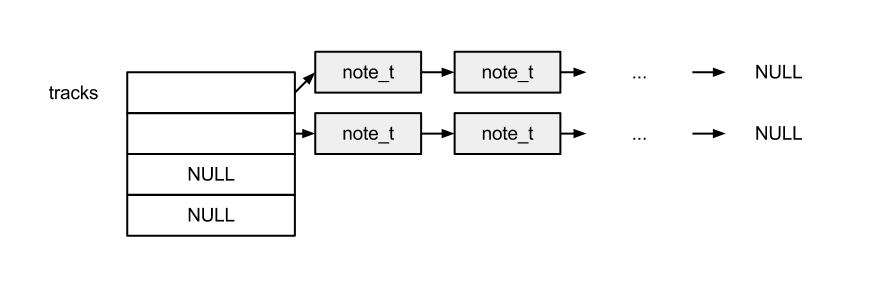
\includegraphics[width=300px]{tracks.png}}
  \caption{Illustration of tracks setup with 2 tracks}
\end{figure}

\subsubsection{Sound Samples}
The 7 different soundsamples are contained within an array of function pointers inside 
the \textbf{interrupt.c} file.
Each function initilizes the tracks array by using the \textbf{set\_track} function.

\subsubsection{Sine Table}
As the abdac interrupt routine is on a deadline, it has to conserve it's computing. Computing a \textbf{sin}
function on every interrupt is wastefull and time-consuming. To make this a constant operation at runtime
a sine table is computed on startup and stored in the \textbf{sine\_table} array in the \textbf{samples.c} file.

\subsection{Waves}

To make sound waves we need some functions producing wave signals. The following waves are implemented
in \textbf{samples.c}.

\begin{figure}[h]
\centering
  \subfigure[Sine wave]{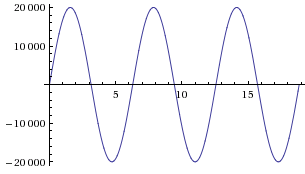
\includegraphics[width=150px]{sine.png}}
  \subfigure[Square wave]{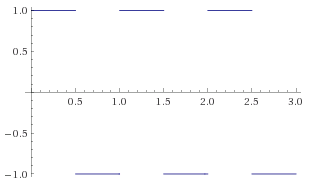
\includegraphics[width=150px]{square.png}}
  \subfigure[Sawtooth wave]{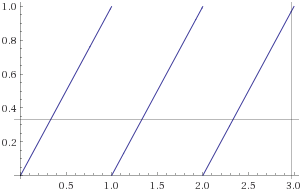
\includegraphics[width=150px]{sawtooth.png}}
  \subfigure[Triangle wave]{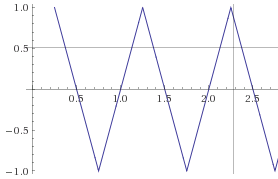
\includegraphics[width=150px]{triangle.png}}
\end{figure}
